\section{Background: Time Series Classification using Untrained Convolutional Kernels}
\label{sec:Background}

We describe a family of time series classifiers which take inspiration from \textbf{random convolutional kernels} in machine learning \cite{Jarrett2009, Pinto2009, Cox2011, Saxe2011, Yosinski2014}: a large number of randomly-generated kernels with fixed weights can capture many relevant features for a downstream classifier. This approach is quite different from \textbf{convolutional neural networks (CNNs)} where kernel weights are learned \cite{Cui2016, Wang2017, Fawaz2019a, Fawaz2019b, Zimmerman2019, InceptionTime, Fawaz2020b}.

\subsection{Classifier Overview}
\label{sec:Overview}

Let $T = \langle t_1, t_2, \ldots, t_n \rangle \in \mathbb{R}^n$ be a time series of length $n$. $T$ can be \textbf{padded} with leading/trailing zeroes as needed. $T$'s \textbf{first-order difference}, $T' = \langle t_i - t_{i-1}| 2 \leq i \leq n \rangle \in \mathbb{R}^{n-1}$, is also a time series.

Let $\omega \in \mathbb{R}^m, m \ll n$ be an ordered sequence of constant values called a \textbf{kernel}. A \textbf{feature map} $T * \omega \in \mathbb{R}^{n-m+1}$ is computed by applying a one-dimensional \textbf{convolution} operator $*$ to $T$ and $\omega$. A convolution $*_d$ with a \textbf{dilation} of $d$ skips every $d-1$ scalar elements of $T$ during the convolution \cite{Yu2015, Bai2018}; when accounting for dilations $T *_d \omega \in \mathbb{R}^{(n-m+1)/d}$.
Fig. \ref{fig:convolutions} illustrates these concepts.

\begin{figure}[tp]
    \centering
        \begin{subfigure}{\linewidth}
      \centering
      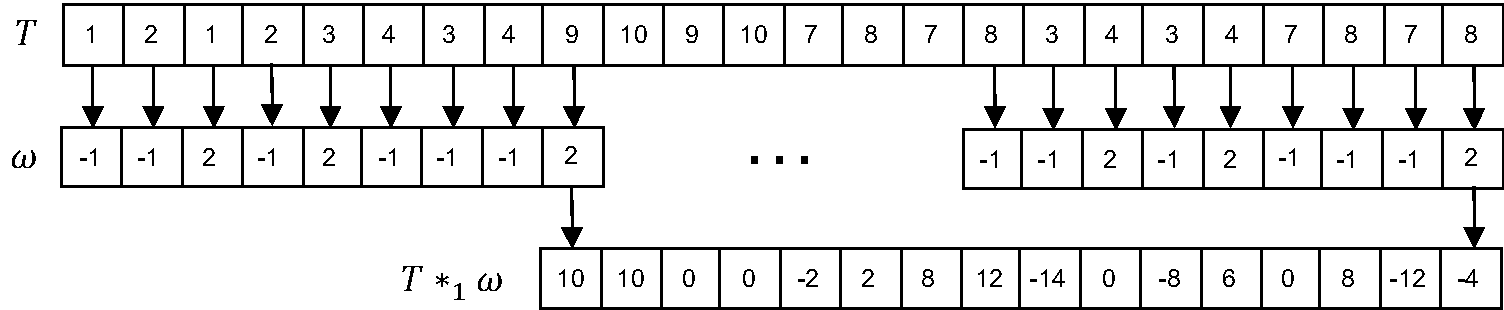
\includegraphics[width=\linewidth]{Figures/conv_d1.pdf}
      \caption{Dilation $d = 1$.}
      \label{fig:conv_d1}
    \end{subfigure}
    \begin{subfigure}{\linewidth}
        \centering
          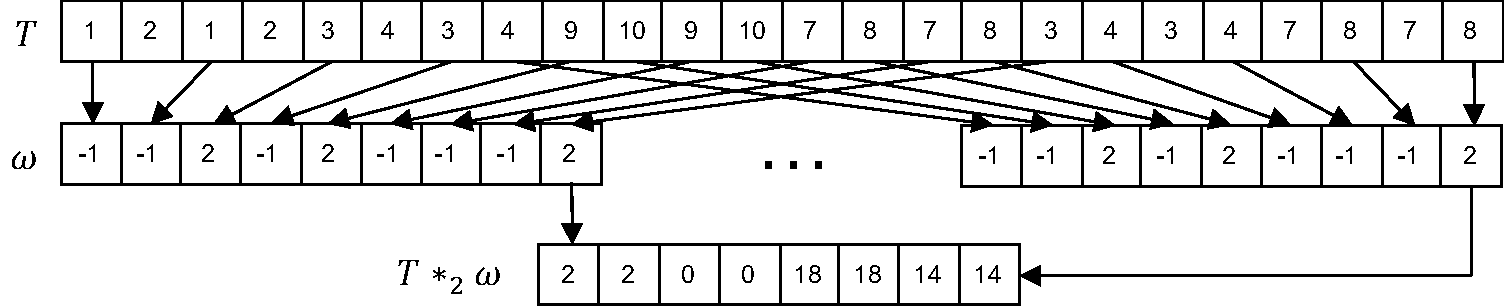
\includegraphics[width=\linewidth]{Figures/conv_d2.pdf}
        \caption{Dilation $d = 2$.}
        \label{fig:conv_d2}
    \end{subfigure}
    \caption{Convolutions with dilations (a) $d = 1$ and (b) $d = 2$.}
    \label{fig:convolutions}
\end{figure}

Let $\Omega = \langle\omega_1, \omega_2, \ldots, \omega_N\rangle \in \mathbb{R}^{Nm}$ be an ordered sequence of kernels. Each kernel is convolved with $T$ using a discrete set of dilation values $D \subset \mathbb{N}^+$ to produce an ordered set of feature maps $T * \Omega = \langle T*_d\omega_i| 1 \leq i \leq N, d \in D\rangle$.

A \textbf{reduction} function $f: \mathbb{R}^{n-m+1} \rightarrow \mathbb{R}$ computes a scalar property of a feature map.
A \textbf{pooling layer} computes the reduction for each feature map: $F(T * \Omega) = \langle f(T*_d\omega_i)| 1 \leq i \leq N, d \in D\rangle$,
 producing a \textbf{feature vector} for a downstream classifier.
Recommended classifiers are \textbf{ridge regression} (for smaller datasets) and \textbf{logistic regression} (for larger datasets) \cite{Rocket}.

\subsection{Dilations}
\label{sec:Dilations}

Computing a convolution using the same kernel but with different dilations captures the pattern at varying scales.
Dilations commonly used include: (1) random dilations; (2) uniformly spaced dilations in $[1, \lfloor 2^p \rfloor]$, where $p = log_2(n-1)/8$; and (3) exponential dilations $\{2^0, 2^1, 2^2, \ldots \}$.

\subsection{Reduction Function}
\label{sec:Reductions}

MiniRocket uses a single reduction function. Given a \textbf{bias} term $b > 0$, the \textbf{(multi-)set of positive values} of convolution $T * \omega$ with bias $b$ is:
\begin{equation}
    PV_b(T * \omega) = \underset{1 \leq i \leq n-m+1}{\{ u_i \in T*\omega|u_i > b \}}
    \label{eq:pv}
\end{equation}
The \textbf{Proportion of Positive Values (PPV)} is:
\begin{equation}
    PPV_b(T*\omega) =\frac{1}{n-m+1}\biggl| PV_b(T*\omega)\biggr|
    \label{eq:ppv}
\end{equation}

\subsection{Convolutional Kernel-based Feature Generators}
\label{sec:Classifiers}

\subsubsection{\textbf{MiniRocket}}
A kernel-based classifier parameterized with kernel length $m = 9$, kernels $\omega \in \{-1, 2\}^9$ with six values of $-1$ and three of $2$ (i.e., $C(9, 3) = 84$ kernels), bias $b$ taken from the convolution output, fixed padding and dilation, and uniformly-spaced dilations with a maximum of $32$ dilations per kernel. MiniRocket uses the PPV reduction function exclusively to generate $\mathtt{\sim}10{,}000$ features: $F_{PPV}(T * \Omega)$.

\subsubsection{\textbf{Hydra}}
An alternative approach that computes histograms as features rather than pooling \cite{Hydra}. Hydra uses kernel length $m = 9$, random kernels $\omega \sim \{\mathcal{N}(0,1)\}^{n-m+1}$, fixed padding, and exponential dilations. Hydra forms $G$ groups of $K$ kernels each. Let $\Omega^{(g)} = \langle \omega_1^{(g)}, \ldots, \omega_K^{(g)} \rangle$ denote the $g^{th}$ kernel group. For each group, Hydra computes convolutions $T *_d \Omega^{(g)}$ and $T' *_d \Omega^{(g)}$ for all $d \in D$.

Consider convolution $T *_d\ \omega_j^{(g)} = \langle x_{1, j}^{(g)}, \ldots, x_{p, j}^{(g)} \rangle$, where $p$ is the number of channels. The \textbf{maximum response} and \textbf{maximum response index} for channel $i$ are:
\begin{equation}
    \mathcal{R}_{max,i}(T *_d \Omega^{(g)}) = \max\limits_{1 \leq k \leq K}(x_{i,k}^{(g)})
    \label{eq:Rmax}
\end{equation}
\begin{equation}
    \mathcal{I}_{max,i}(T *_d \Omega^{(g)}) = \argmax\limits_{1 \leq k \leq K}(x_{i,k}^{(g)})
    \label{eq:Imax}
\end{equation}
The \textbf{maximum channel set} for kernel $\omega_j^{(g)}$ is $\mathcal{C}_{max}(\omega_j^{(g)}) = \{i|\ \mathcal{I}_{max,i}(T *_d \Omega^{(g)}) = j\}$.
Minimum responses and channel sets are defined analogously using $-\Omega^{(g)}$.

Hydra defines a \textbf{hard count} as the number of channels for which each kernel computes the maximum response, and a \textbf{soft count} as the sum of those maximum responses. The \textbf{minimum hard count histogram} and \textbf{maximum soft count histogram} are:
\begin{equation}
    H_{min}(T *_d \Omega^{(g)}) = \left\langle \biggl|\mathcal{C}_{min}(\omega_j^{(g)})\biggr|\ |\ 1 \leq j \leq p \right\rangle
    \label{eq:Hmin}
\end{equation}
\begin{equation}
    S_{max}(T *_d \Omega^{(g)}) = \left\langle \sum_{i\in \mathcal{C}_{max}(\omega_j^{(g)})}x_{i,j}^{(g)}\ |\ 1 \leq j \leq p \right\rangle
    \label{eq:Smax}
\end{equation}
Hydra generates features $H_{min}(T *_d \Omega^{(g)}) \cdot S_{max}(T *_d \Omega^{(g)})$ for $1 \leq g \leq G, d \in D$.

\subsection{Regression Classifier}
\label{sec:regression}

Let $F(T*\omega) \in \mathbb{R}^{\left|D\right|NM}$ be the feature vector produced by one of the kernel-based classifiers, \textbf{z-score normalized} to $\overline{F(T*\omega)}$, and provided as input to ridge regression or logistic regression \cite{Rocket}. Both are linear classifiers with response function
$\overline{F(T*\omega)}\cdot W \in \mathbb{R}$, where $W \in \mathbb{R}^{\left|D\right|NM}$ is the set of trained weights.

Let $C = \langle C_1, C_2, \ldots C_P\rangle$ be the set of classes. The regression classifier comprises $P$ independent linear classifiers with weights $\langle W_1, W_2, \ldots, W_P \rangle$, each predicting the probability that $T$ belongs to each class. The predicted class is:
\begin{equation}
    j = \argmax\limits_{1 \leq i \leq P}(\overline{F(T*\omega)}\cdot W_i).
    \label{eq:predicted_class}
\end{equation}

